\documentclass[10pt]{article}
\usepackage[utf8]{inputenc}
\usepackage[T1]{fontenc}
\usepackage{amsmath}
\usepackage{amsfonts}
\usepackage{amssymb}
\usepackage[version=4]{mhchem}
\usepackage{stmaryrd}
\usepackage{bbold}
\usepackage{graphicx}
\usepackage[export]{adjustbox}
\graphicspath{ {./images/} }

\begin{document}
\section*{Introduction to Stochostic Processes}
We will present bosic results from the therey of stochastic processes. Rigowns definitions and proofs need notions of measure theory that we do not introduce nor assume. therefore, this introduction will necessarily be non-rigorous, with some loosemess in the definitions and some inaccuracies in the proofs. There are many books which can give you the mathematical nigour that is necessary for obtainig a full understanding of stochastic processes. These notes, instead, wish to provide enough awarmess to make you able to use the tools in applied problems (in physics, biology, finance...).

In the following we will connect the diffusion equation to the most important continuous stochastic process: the Brownion motion (or Wiener Process). This is the bosis for building up stochastic differential equations whose solutions have continuous trajectories. These are crucial for defining stochastic models that will be used in several fields of physics.

Useful books: "2atrod. to Stoch. Colculus with Applic., F.C. Kleboner, Imperial P.

\begin{itemize}
  \item An antrod. to SDEs, Lawzence $C$. Evens, AMS
  \item Stoch. Proc. and Applications, G. A. Pavliotis, Springer
  \item Stoch. The thods, C. Gardiner, Springer
  \item Stoch. Diff. Eq., B. Dksendol, Springer
  \item Stoch. proc. in Physics and chemistry, N.G. von tampen.
\end{itemize}

Example: Tossing a coin\\
Let's assume that we ten a cain 3 times (heads $\rightarrow 0$, tails $\rightarrow 1$ ) and we ask: what is the sum of the 3 tosses? We define a function sample spece (the realization) state spece (what we measure)\\
$Y: \Omega=\left\{\begin{array}{ccc}(0,0,0), & (0,0,1) \ldots & (1,1,1) \\ \omega_{1} & \omega_{2} & \omega_{8}\end{array}\right\} \longrightarrow E=\left\{\begin{array}{ccc}0,1, & 2,3 \\ \uparrow & \uparrow \\ y & \uparrow & \uparrow \\ y & y_{2} & y_{3}\end{array}\right\}$\\
and intraduce probabilities $\mathbb{P}: \Omega \rightarrow[0,1]$ s.t. $\sum_{\omega} P(\omega)=1$; we define $P_{i}=\sum_{\omega: Y(\omega)=y_{i}} \mathbb{P}(\omega)=P\left(Y=y_{i}\right)$. More generally, we con define probabilities\\
for all sets of type $Y^{-1}(B) \subseteq \Omega$, for $B \subseteq E$. This means that $Y$ is a measurable function and this defines a rondom variable.\\
When $\Omega$ is finite, $Y(\Omega)$ is finite and we con always define a zondom variable as before. We con also define the expectation es

$$
E(Y)=\sum_{\omega \in \Omega} Y(\omega) \mathbb{P}(\omega)=\sum_{i=1}^{4} y_{i} P\left(Y=y_{i}\right)=\sum_{i=1}^{4} y_{i} P_{i}
$$

When $\Omega$ is an uncountable set, the definition of z.v. needs much care, because we have to moke sure that $x$ is still a measurable function. In simple terms $x$ is a real-valued zondom variable when we con assign probabilities to sets (colled events) of the form $\{x \leq x\}$ and $\{a<x \leq b\}$ for $x, a, b \in \mathbb{R}$.\\
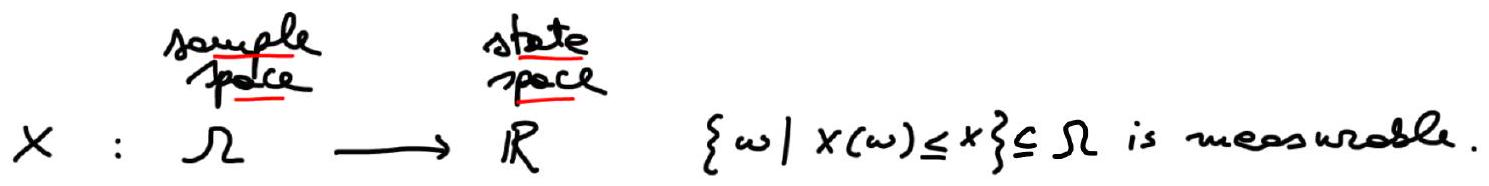
\includegraphics[max width=\textwidth, center]{2025_10_17_79731b7d4e7690819b81g-02}

More precisely, a zondom variable is a measurable function for which the preimage of any Borel set in $\mathbb{R}$ is a measuroble set in $\Omega$.

\section*{Definition of stochestic process}
A stochostic poces is a callection of random voriables $\{x(t, \omega), t \in T, \omega \in \Omega\}$, where $T$ is an ordered set (itime") (it can be either discrete, $T=\mathbb{Z}_{+}$, or continuous, $T=\mathbb{R}^{+}$). For cach fixed time $t \in T, x(t, \omega)$ indicates a sondom variable from $\Omega$ (rigorously, from the probability space $(\Omega, \sigma, \mathbb{P})$ ) to $E$ (rigorously, $E$ is a measurable spece equipped with a $\sigma$-algebse; for instance, $E=\mathbb{R}^{d}$ and the $\sigma$-regebra is the one of Bovel sets; we need a "filtroction" as well).\\
$\Omega$ is the common somple space, $E$ is the state spece of the process.\\
For each fixed $\omega \in \Omega, x(t, \omega)$ is a function of time $t$ that is called a sample path a stochastic valization of the process. We will usually omit the $w$-dependence, i.e., we write $x(t)$.

\section*{Examples:}
\begin{enumerate}
  \item Let $E=\{0,1,-1\}$ be the state space of a stoch-proc $x$ and let $T=\{0,1,2,3\}$ be the (discrete) time. There are then $3^{4}$ somple peths, thus $|\Omega|=3^{4}=81$.\\
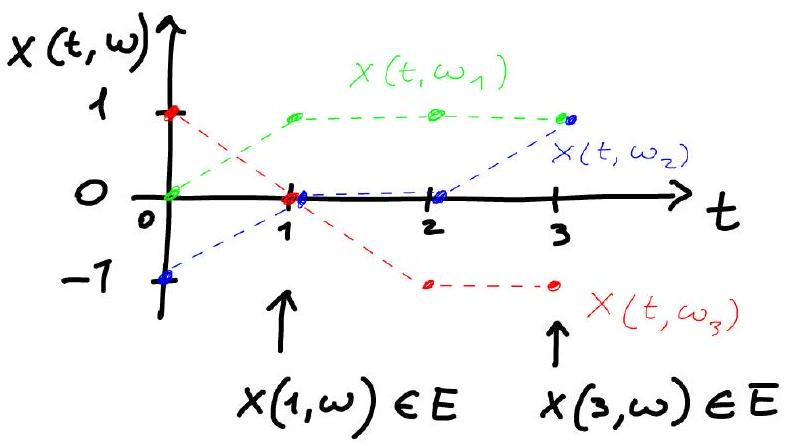
\includegraphics[max width=\textwidth, center]{2025_10_17_79731b7d4e7690819b81g-03}
\end{enumerate}

In this example we can enumerote all the 81 trajectories. This is not possible if $E$ is an uncountable set.\\
2) The sondom walk process in discrete time has\\
$E=\mathbb{Z}$ (position) and $T=\mathbb{N}$ (time), thus $x(t, \omega)$ indicates a stochastic realization (or trajectory) as a function of time $t$.\\
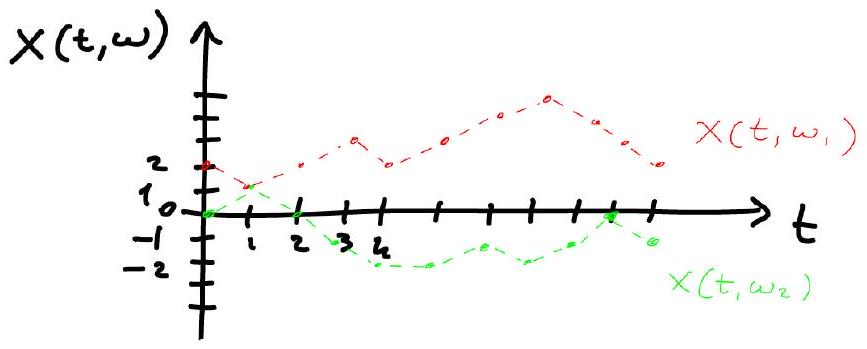
\includegraphics[max width=\textwidth, center]{2025_10_17_79731b7d4e7690819b81g-03(1)}

Here we get infinitely countable trajectories ( $|\Omega|=\left.|\mathrm{z}|\right|^{\mathrm{w}}$ )\\
3) The position of a Browmion perticle is described by the Brownion process for which $T=\mathbb{R}^{+}$and $E=\mathbb{R}$ and one sample poth is $x(t, \omega)$\\
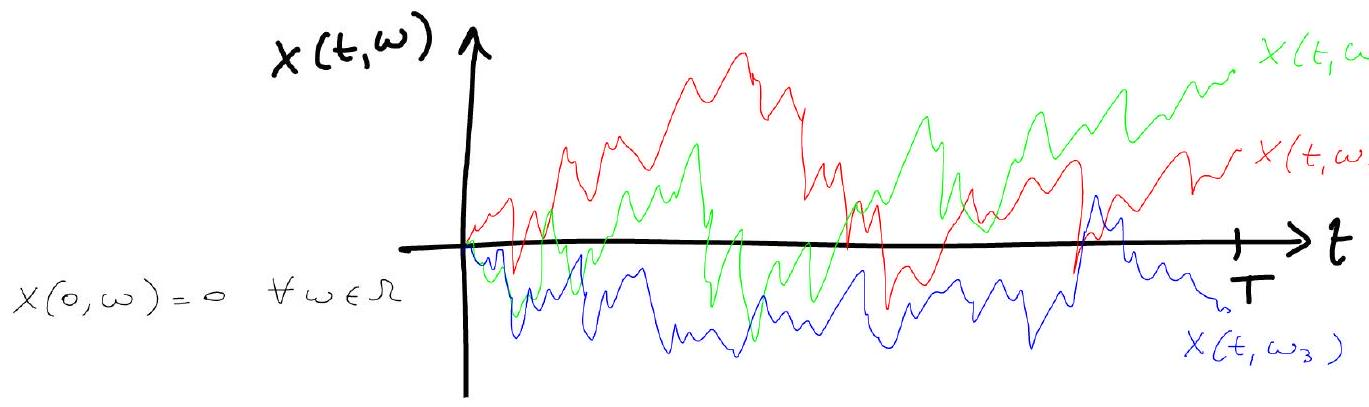
\includegraphics[max width=\textwidth, center]{2025_10_17_79731b7d4e7690819b81g-03(2)}\\
here every poth is a continuous function of time $x(t, \omega) \in C^{0}([0, T])$

In the following we will omit $w$ and we will simply write $x(t)$, because what we "observe" is the volue $x \in E$ at some time $t$ and not $\Omega$.

Notice that in these examples we have not defined a prob.measure, which is not needed for defining a random variable.

One of the most important stochastic processes is the Brownian process/motion or Wiener process.\\
This can be used to describe the motion of a heary perticle in a fluid made of light particles, which callide with it randomly. For the time being, we will not laok into how good this process is for empinical Brownion particles.

Brownion motion (or Wiener process)\\
A standord Brownion motion in $1-d, B(t)$, is a real-valued stoch. process $\left(E=\mathbb{R}, T=\mathbb{R}^{+}\right)$for which\\
(A) $B(0)=0 \quad($ a.s. , namely, Prob. $\{w(0)=0\}=1)$\\
(B) For any $0 \leqslant s<t<\infty, B(t)-B(s)$ is normally distributed, that is $B(t)-B(s) \underset{\text { sompled from }}{\sim} N(0, t-s)=\frac{1}{\sqrt{2 \pi(t-s)}} e^{-\frac{\Delta x^{2}}{2(t-s)}}$ (mean 0 and variance $t-s$ )\\
(c) For all times $0=t_{0}<t_{1}<t_{2}<\ldots<t_{m}$ the imerements $\Delta B_{i}:=B\left(t_{i}\right)-B\left(t_{i-1}\right)$ are independent (of each other)

Some important properties:

\begin{enumerate}
  \item Stationarity of increments: notice that, if we write $t=s+\Delta t$, then from (B) we get
\end{enumerate}

$$
B(s+\Delta t)-B(s) \sim N(0, \Delta t)
$$

which means that the distribution of $B(s+\Delta t)-B(s)$ does not depend on $S$. This means that the imcrements are not only independent, but also stationary, namely they depend only on $\Delta t: \Delta B=B(s+\Delta t)-B(s) \sim B(\Delta t)$.

Since $\operatorname{Ver}[B(\Delta t)]=\Delta t$, we expect that $|\Delta B|=|B(\Delta t)| \simeq \sqrt{\Delta t}$ as $\Delta t \rightarrow 0^{+}$. This will be crucial in the future, in many colculations.\\
2) Connection with the diffusion equation

We have seen that the fundamental solution of the diffusion $\varphi$. ( $D=1$ )

$$
\left\{\begin{array}{cc}
\partial_{t} w(x, t)=\frac{1}{2} \partial_{x}^{2} w(x, t) & x \in \mathbb{R}, t>t_{0} \\
w\left(x, t_{0}\right)=\delta\left(x-x_{0}\right) & t=t_{0}
\end{array}\right.
$$

is the propogator of the Brownion motion:


\begin{equation*}
w\left(x, t \mid x_{0}, t_{0}\right)=\frac{1}{\sqrt{2 \pi\left(t-t_{0}\right)}} e^{-\frac{\left(x-x_{0}\right)^{2}}{2\left(t-t_{0}\right)}} \tag{1}
\end{equation*}


which is the one we use in (B). So from time to time the procen evolves with the propaptor (1) and with stationary independent increments.\\
3) Correlation function

The average will be indicated either with $\langle\cdots\rangle$ or with $\mathbb{E}(\cdots)$. Let $0 \leqslant s \leqslant t:$ from (B) $\mathbb{E}[B(s)]=0, \mathbb{E}\left[B(s)^{2}\right]=s$. Then

$$
\begin{aligned}
\mathbb{E}[B(t) B(s)]= & \mathbb{E}[(B(s)+B(t)-B(s)) B(s)]= \\
= & \mathbb{E}\left[B(s)^{2}+(B(t)-B(s)) B(s)\right]= \\
= & \mathbb{E}\left[B(s)^{2}\right]+\mathbb{E}[(B(t)-B(s)) B(s)]= \\
& \downarrow(B) \quad \text { depends on t-s only } \\
= & s+\underbrace{\mathbb{E}[(B(t)-B(s))}_{=0}] \underbrace{\mathbb{E}[B(s)]}_{=0}(B)
\end{aligned}
$$

Thus for $s, t \geqslant 0$\\
(2) $\mathbb{E}[B(t) B(s)]=\min (t, s)$

Exercizes: i) (Orustein-Chlembeck process). Define $V(t)=e^{-t} B\left(e^{2 t}\right)$ where $B(t)$ is a Brownion process. Show that $\mathbb{E}[V(t)]=0$ and $\mathbb{E}[V(t) V(s)]=e^{-|t-s|}$.\\
ii) (Brownion bridge). Define $V(t)=T B(t)-t B(T)$ for any $t \in[0, T]$, where $B(t)$ is a Brownion process. Show that $\mathbb{E}[V(t)]=0$ and $\mathbb{E}[V(t) V(s)]=T^{2} \min (t, s)-T t s$ for any $t, s \in[0, T]$.\\
iii) Show that $\mathbb{E}\left[e^{i \lambda B(t)}\right]=e^{-\frac{\lambda^{2} t}{2}}$ for $t \geqslant 0, B(t)$ B.m.\\
iv) With the help of the Law of lage numbers and $B(t)=\sum_{i}^{t} \Delta B_{i}$, show that $\lim _{t \rightarrow \infty} \frac{B(t)}{t}=0$.\\
4) Rescaling. The process $z(t)=\frac{1}{\sqrt{c}} B(c t), c>0$, is a Brownion motion that is distributed like $B(t)$, another Brownion motion. (Verify $(A),(B)$ and $(C)$ ). Also:

$$
\mathbb{E}\left[e^{i \lambda z(t)}\right]=\mathbb{E}\left[e^{i \lambda \frac{1}{\sqrt{c}} B(t c)}\right]=e^{-\frac{\lambda^{2}}{2 c} t c}=e^{-\frac{\lambda^{2} t}{2}}=\mathbb{E}\left[e^{i \lambda B(t)}\right] .
$$

\begin{enumerate}
  \setcounter{enumi}{4}
  \item Inversion. The process $z(t)=t B\left(\frac{1}{t}\right)$ for $t>0$ and $z(0)=0$ is distributed like $B(t)$, another B.m.
\end{enumerate}

$$
\mathbb{E}\left[e^{i \lambda z(t)}\right]=\mathbb{E}\left[e^{i \lambda t B\left(\frac{1}{t}\right)}\right]=e^{-\frac{\lambda^{2}}{2} t^{2} \cdot \frac{1}{t}}=e^{-\frac{\lambda^{2} t}{2}}=\mathbb{E}\left[e^{i \lambda B(t)}\right]
$$

Notice that $\lim _{t} \frac{z(t)}{t}=\lim _{t} B\left(\frac{1}{t}\right)=0$ as in (iv).\\
6) Time reversal. Define $z(t)=B(T)-B(T-t)$ for any $t \in[0, T]$. Then $Z(t)$ and $B(t)$ have the same distrib.

Properties of the trajectories of the Brownian motion. These are hard to prove rigorously, but somehow easy to guess. Let's consider the zotio $\frac{\Delta B}{(\Delta t)^{\alpha}}$ where $\Delta t=t_{2}-t_{1}>0, \alpha>0$ and $\Delta B=B\left(t_{2}\right)-B\left(t_{1}\right)$. What happens to this ratio as $\Delta t \rightarrow 0^{+}$? Take some $k \in \mathbb{R}^{+}$:


\begin{align*}
& P\left(\left|\frac{\Delta B}{\Delta t^{\alpha}}\right| \leqslant k\right)=P\left(|\Delta B| \leqslant k \Delta t^{\alpha}\right)=\int_{-k(\Delta t)^{\alpha}}^{k(\Delta t)^{\alpha}} d x \frac{e^{-\frac{x^{2}}{2 \Delta t}}}{\sqrt{2 \pi \Delta t}}= \\
& =\frac{2}{\sqrt{2 \pi \Delta t}} \int_{0}^{k(\Delta t)^{\alpha}} d x e^{-\frac{x^{2}}{2 \Delta t}}=\frac{2}{\sqrt{2 \pi}} \int_{0}^{k(\Delta t)^{\alpha-1 / 2}} d z e^{-z^{2} / 2}  \tag{3}\\
& z=\frac{x}{\sqrt{\Delta t}}
\end{align*}


Here are the consequences:

\begin{enumerate}
  \item $0<\alpha<\frac{1}{2}$, as $\Delta t \rightarrow 0^{+}, \quad P\left(\left|\frac{\Delta B}{\Delta t^{\alpha}}\right| \leqslant k\right) \rightarrow 1$ zegardless of $k$. This tells us that as $|t-s| \rightarrow 0^{+}$
\end{enumerate}

$$
|B(t)-B(s)| \leqslant \text { const }|t-s|^{\alpha}
$$

which means that Brownion trajectories are Hölder continuous for any $0<\alpha<\frac{1}{2}$. This con be proven rigorously.\\
2) $\alpha=1$ (or $\frac{1}{2}<\alpha \leqslant 1$ ), as $\Delta t \rightarrow 0^{+}, P\left(\left|\frac{\Delta B}{\Delta t}\right| \leqslant k\right) \rightarrow 0 \quad \forall k \in \mathbb{R}^{+}$

This tells us that the Browmian trajectories are nowhere differentiable. This is expected because if $|\Delta B| \sim \sqrt{\Delta t}$, then $\frac{|\Delta B|}{\Delta t} \sim \frac{1}{\sqrt{\Delta t}}$ and hence $\lim _{t \rightarrow 0^{+}} \frac{|\Delta B|}{\Delta t} \rightarrow \infty$.\\
This is related to the fact that B.m. has no memory of the post (see the Markov property below).

We con add a drift $\mu$ and change the diffusion coefficient of a Brownian motion with no difficulty. We define a Brownion motion with drift $\mu$ and variance $D$ the process\\
(4) $x(t)=x_{0}+\mu t+\sqrt{D} B(t)$

Verify that $\mathbb{E}[x(t)]=x_{0}+\mu t$ and $\operatorname{Var}[x(t)] \equiv \mathbb{E}\left[(x(t)-\mathbb{E}[x(t)])^{2}\right]=D$. Notice that $x(t)$ sotisfies the stochastic differential equation:\\
(5) $d x(t)=\mu d t+\sqrt{D} d B(t)$

How to simulate a very simple SDE (including B.m.) We wish to generate a path of ey. (5), starting from $x(0)=x_{0}$. Beconse $\Delta B \sim B(\Delta t) \sim \sqrt{\Delta E} B(1)$ for finite times $t_{0}=0<t_{1} \cdots <t_{m-1}<t_{m}$ we can write (5) as ( $\Delta t=t_{i}-t_{i-1}$ )\\
(6)

$$
\begin{aligned}
x\left(t_{i}\right) & =x\left(t_{i-1}\right)+\mu \Delta t+\sqrt{D \Delta t} \varepsilon_{i} \\
x(0) & =x_{0}
\end{aligned} \quad i=1,2, \ldots, n
$$

where $\varepsilon_{i} \sim N(0,1)$. Notice that we use a sequence of $n$ independent and identically distributed zondow voriables $\left\{\varepsilon_{i}\right\}$ drawn from $N(0,1)$ because at every time step we add a random value that is independent of all values that were colculated before (indep. of $x, t, \mu, D \ldots$ ). Of course, $\mu=0 D=1$ and $x_{0}=0$ generate a standard Brownian motion as defined in $(A),(B)$ and $(c)$.

\section*{Markov processes}
Let us focus on a stochastic process for which we can the a set of ordered fines, i.e. $t_{0}<t_{1}<t_{2} \cdots<t_{m}$ and there exists a conditional prob. deusity funct. at time $t_{n}$, namely $p_{1 \mid n-1}\left(x_{n}, t_{n} \mid x_{n-1}, t_{n-1} ; \ldots ; x_{1}, t_{1} ; x_{0}, t_{0}\right)$.\\
This PDF tells us what is the prob. of observing $x_{\mu}$ at time $t_{m}$, if we know what happened to the process at previous times; we really know the actual values that occurred, not only their propobilities. This is quite a lot of imporeation and besically it means that, if we want to make a prediction on what is going to happen in the future, we have to know all that happened in the post. However, in some situations the effect of the post con be neglected. On porticular, if it happens that for any $n=1,2 \ldots$\\
(7) $p_{1 / m-1}\left(x_{m}, t_{m} \mid x_{m-1}, t_{m-1} ; \ldots ; x_{1}, t_{1} ; x_{0}, t_{0}\right)=p_{1 / 1}\left(x_{m}, t_{m} \mid x_{m-1}, t_{m-1}\right)$

Then we soy that the stochastic process is a Markov process. This means that predictions at time $t_{n}$ only depend on what happened at time $t_{n-1}$ and not on the whole his tory of the process. The polf $P_{111}$ is called trousition probability or propegetor.

A Makov process con be fully defined by two functions: the propagator $p_{111}$ and the initial distribution $p_{1}\left(x_{0}, t_{0}\right)$.

Indeed the 3-point joint PDF for a Markov process is $\left(t_{0}<t_{1}<t_{2}\right)$ :\\
$P_{3}\left(x_{2} t_{2} ; x_{1} t_{1} ; x_{0} t_{0}\right)=P_{112}\left(x_{2} t_{2} \mid x_{1} t_{1} ; x_{0} t_{0}\right) P_{2}\left(x_{1} t_{1} ; x_{0} t_{0}\right)=$\\
(8) $=p_{1 / 1}\left(x_{2} t_{2} \mid x_{1} t_{1}\right) \quad$ Markol/property

$$
=P_{1 / 1}\left(x_{2} t_{2} \mid x_{1} t_{1}\right) P_{1 / 1}\left(x_{1} t_{1} \mid x_{0} t_{0}\right) P_{1}\left(x_{0} t_{0}\right)
$$

Therefore we can find iteratively\\
(9)

$$
p_{n}\left(x_{n} t_{n} ; x_{n-1} t_{n-1} ; \ldots ; x_{1} t_{1} ; x_{0} t_{0}\right)=\prod_{i=1}^{n} p_{1 / 1}\left(x_{i} t_{i} \mid x_{i-1} t_{i-1}\right) p_{1}\left(x_{0} t_{0}\right)
$$

this property makes Markor processes much more amenoble to analytical calculations than non-Markov ones.

The Chopman-Kolmogorov equation\\
Not all functions can be used as propogators for Morkov processes, nor an initial distribution $p_{1}$ can be arbitrong. These two functions must sotisfy two indentities, one of which is the $C_{-}-K$. equation.

From the L.H.S. of op. (8), if we integrate wrt $x$,

$$
\int d x_{1} p_{3}\left(x_{2} t_{2} ; x_{1} t_{1} ; x_{0} t_{0}\right)=p_{2}\left(x_{2} t_{2} ; x_{0} t_{0}\right)
$$

from the R.H.S., unstead

$$
=\int d x_{1} p_{1 / 1}\left(x_{2} t_{2} \mid x_{1} t_{1}\right) p_{1 / 1}\left(x_{1} t_{1} \mid x_{0} t_{0}\right) p_{1}\left(x_{0} t_{0}\right)
$$

but $p_{2}\left(x_{2} t_{2} ; x_{0} t_{0}\right)=p_{1 / 1}\left(x_{2} t_{2} \mid x_{0} t_{0}\right) p_{1}\left(x_{0} t_{0}\right)$, becouse of the Markov property, so\\
(10)\\
$p_{1 / 1}\left(x_{2} t_{2} \mid x_{0} t_{0}\right) p_{1}\left(x_{0} t_{0}\right)=\int d x_{1} p_{1 / 1}\left(x_{2} t_{2} \mid x_{1} t_{1}\right) p_{1 / 1}\left(x_{1} t_{1} \mid x_{0} t_{0}\right) p_{1}\left(x_{0} t_{0}\right)$\\
hence, for any $t_{2}>t_{1}>t_{0}$\\
(11) $\quad p_{111}\left(x_{2} t_{2} \mid x_{0} t_{0}\right)=\int d x_{1} p_{1 / 1}\left(x_{2} t_{2} \mid x_{1} t_{1}\right) p_{1 / 1}\left(x_{1} t_{1} \mid x_{0} t_{0}\right)$\\
this is the Chapman-Kohngorov equation (octually, identity), which must be sotisfied by any propagator/trousition probab. If we further integrate ef. (10) w.r.t. $x_{0}$ we get

$$
\int d x_{0} p_{1 / 1}\left(x_{2} t_{2} \mid x_{0} t_{0}\right) p_{1}\left(x_{0} t_{0}\right)=p_{1}\left(x_{2} t_{2}\right)
$$

and

$$
\int d x_{0} p_{1 / 1}\left(x_{1} t_{1} \mid x_{0} t_{0}\right) p_{1}\left(x_{0} t_{0}\right)=p_{1}\left(x_{1} t_{1}\right)
$$

we obtain, for $t_{2}>t_{1}$,\\
(12) $\quad p_{1}\left(x_{2} t_{2}\right)=\int d x_{1} p_{1 \mid 1}\left(x_{2} t_{2} \mid x_{1} t_{1}\right) p_{1}\left(x_{1} t_{1}\right)$\\
this is the $2^{\text {nd }}$ ep. (identity) for a Markor process. Therefore $P_{1}$ and $P_{1 / 1}$ are connected to each other.\\
It can be proven that any two non-negative functions that setisfy eps. (11) and (12) define a Markor process.

\section*{Stationary Mankov Process}
If $p_{1}$ is independent of time and equal to the equilibrium dirtribution of the stochastic process, and $p_{1 / 1}$ depends only on the time difference $\left|t_{2}-t_{1}\right|$, then the process is a stationary Monter process.

The Brownian motion is a Markor process\\
This property essentially follows from the independence of the increments and it can be proven in different ways. On our context, we con use $\varphi$. (1), i.e. the propogotor\\
(13) $P_{11}\left(x_{1}, t_{1} \mid x_{0}, t_{0}\right) \equiv W\left(x_{1}, t_{1} \mid x_{0}, t_{0}\right)=\frac{1}{\sqrt{2 \pi\left(t_{1}-t_{0}\right)}} e^{-\frac{\left(x_{1}-x_{0}\right)^{2}}{2\left(t_{1}-t_{0}\right)}}$\\
and show that ep. (11) is satisfied by direct integration. Also, if you take $P_{1}\left(y_{1}, t_{1}=0\right)=\delta\left(y_{1}\right)$ you get from ep. (12) $p_{1}\left(y_{2}, t_{2}\right)=\frac{1}{\sqrt{2 \pi F_{2}}} e^{-y_{2}^{2} / 2 t_{2}}$. These generate a nom-stationaly Markov process.

\section*{Exercises:}
\begin{enumerate}
  \item Show that the Poisson process defined by
\end{enumerate}

$$
P_{1 / 1}\left(x_{2} t_{2} / x_{1} t_{1}\right)=\frac{\left(t_{2}-t_{1}\right)^{x_{2}-x_{1}}}{\left(x_{2}-x_{1}\right)!} e^{-\left(t_{2}-t_{1}\right)} \quad t_{2}>t_{1}
$$

and $P_{1}(n, 0)=\delta_{n, 0} \Rightarrow P_{1}(n, t)=\frac{t^{n}}{n!} e^{-t}$ is a (non-stationary) Markov process.\\
2) Show that for $x, y= \pm 1$ the function

$$
P_{1 / 1}\left(x t \mid y t^{\prime}\right)=\frac{1}{2}\left[1+e^{-2 \gamma\left(t-t^{\prime}\right)}\right] \delta_{x y}+\frac{1}{2}\left[1-e^{-2 \gamma\left(t-t^{\prime}\right)}\right] \delta_{x,-y}
$$

sotisfies ey. (11).\\
3) Show that the process defined by

$$
P_{1}(x)=\frac{1}{\sqrt{2 \pi}} e^{-x^{2} / 2}
$$

$p_{1 / 1}\left(x t \mid y, t^{\prime}\right)=\frac{1}{\sqrt{2 \pi\left(1-e^{-2\left|t-t^{\prime}\right|}\right)}} \exp \left[-\frac{\left(x-y e^{-\left|t-t^{\prime}\right|}\right)^{2}}{2\left(1-e^{-2\left|t-t^{\prime}\right|}\right)}\right]$ is a stationary Markov process. This is called the O.U. proc.


\end{document}